
\chapter{Sound absorption}
	\begin{wrapfigure}[10]{l}{6cm}
	\vspace{-5mm}
	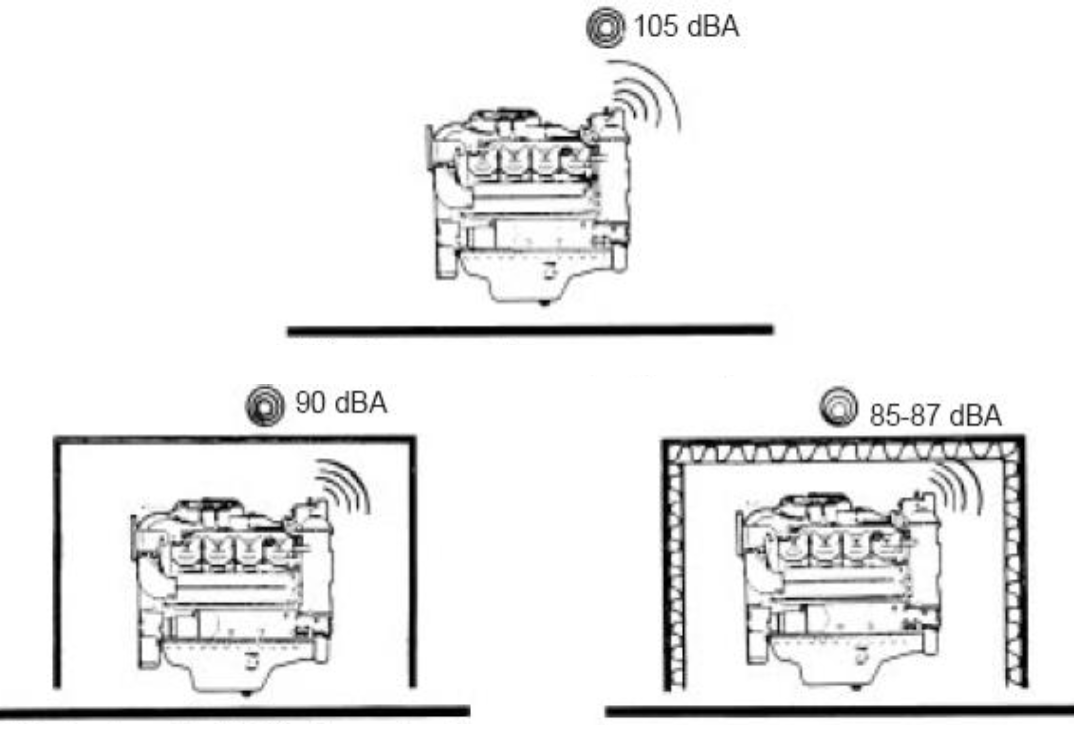
\includegraphics[scale=0.2]{acoustics/ch4/1}
	\captionof{figure}{}
	\label{fig:4.1}
	\end{wrapfigure}
	How are we going to limit the sound emitted from the engine? They use now steel panel, the heaviest material is the best. If we excite at the proper frequency we can have resonance, how to do not to have the proper frequency? The sound amplification doesn't result from the panel vibration, but by the sound wave amplifying each other. We have to manage the inside of the panel with sound absorbing material, it transfers acoustic energy into heat, avoiding the reflection of sound into the box. For example in glasswool the vibration of the molecules are creating heat. On the figure, the second case the sound is insulated with a huge mass, but the sound remains high in the box, in the third case we limit also the sound in the box. 
	
\section{Absorption and reflection coefficients}
	
	\begin{wrapfigure}[10]{r}{3cm}
	\vspace{-5mm}
	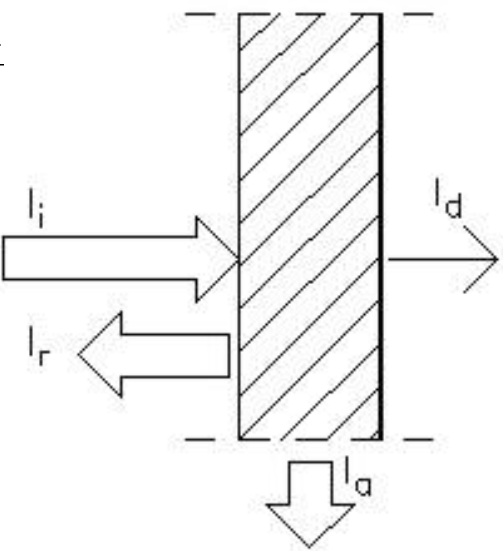
\includegraphics[scale=0.2]{acoustics/ch4/2}
	\captionof{figure}{}
	\label{fig:4.2}
	\end{wrapfigure}
	Let's study what happens when interacting with a wall. We do an energy balance, part of the incident energy is reflected, transmitted or absorbed. By the division we get the sum of three ratios, r d and a:
	
	\begin{equation}
	I_i = I_r + I_d + I_a \qquad \Rightarrow 1 = r + d + a 
	\end{equation}
		
	 We are assuming in this chapter that the $I_d$ is small. For example for a very poor insulation of 20 dB (extremely low), $d = 0.01$. The amount of absorbed energy is higher. For glasswool for example, $a = 0.99$. $d$ can be neglected. 
	 \ \\
	 
	\begin{wrapfigure}[9]{l}{3cm}
	\vspace{-5mm}
	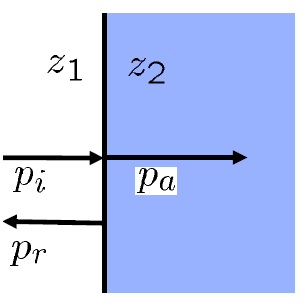
\includegraphics[scale=0.3]{acoustics/ch4/3}
	\captionof{figure}{}
	\label{fig:4.3}
	\end{wrapfigure}
	Now if we have the r we have the a. Let's look to 2 materials: air impedance $z_1 = \rho c =400$ and the second with a second $z_2$, of higher order of magnitude. What will be the different pressures? Let's write the pressure and velocity balance on the interface:
	
	\begin{equation}
	p_i(0,t)+ p_r(0,t) = p_a(0,t), \qquad v_i(0,t) + v_r(0,t) = v_a(0,t).
	\end{equation}
	
	By definition of the impedance $z = \rho c = p/v$, this allows to rewrite the velocity balance as:
	
	\begin{equation}
	\frac{p_i(0,t)}{z_1} + \frac{p_r(0,t)}{z_1} = \frac{p_a(0,t)}{z_2}.
	\end{equation}
	
	By eliminating $p_a$ in the pressure balance we have: 
	
	\begin{equation}
	p_i(0,t)+ p_r(0,t) = \frac{z_2}{z_1} [p_i(0,t)+ p_r(0,t)] \qquad \Rightarrow \frac{p_r}{p_i} = \frac{z_2 - z_1}{z_2 + z_1}.
	\end{equation}
	
	Using the same trick cancelling the $p_r$, we get:
	
	\begin{equation}
	\frac{p_a}{p_i} = \frac{2z_2}{z_2 + z_1}.
	\end{equation}
	 
	We know that $I = p^2/\rho c$, let's use this to determine the ratios:
	
	\begin{equation}
	r = \frac{I_r}{I_i} = \frac{p_r^2/z_1}{p_i^2 z_1} =  \left( \frac{z_2 - z_1}{z_2 + z_1} \right) ^2 \qquad a = \frac{I_a}{I_i} = \frac{p_r^2z_1}{p_i^2 z_2} =  \frac{4z_1 z_2}{(z_2 + z_1)^2}.
	\end{equation} 
	
	\begin{wrapfigure}[9]{l}{5cm}
	\vspace{-5mm}
	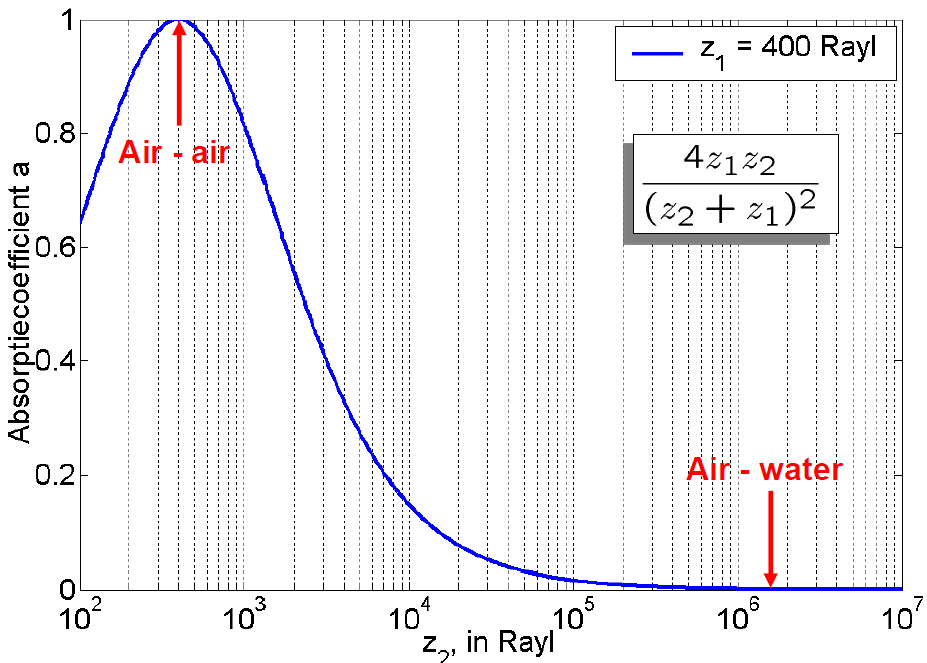
\includegraphics[scale=0.2]{acoustics/ch4/4}
	\captionof{figure}{}
	\label{fig:4.4}
	\end{wrapfigure}
	What will happen for r and a for a very large $z_2$ and small $z_1$ is that $r=1$ and the $a= \frac{4z_1}{z_2}$. \textbf{Everything is reflected}. If the impedances are equal we have the contrary $\Rightarrow$ \textbf{absorption}. The conclusion is that when the impedances are close to each other, the sound is absorbed and when they are different there is a lot of reflection. This is illustrated for the particular case of $z_1$ = air on \autoref{fig:4.4}. 
	
	\ \\\\
	
	We want to know how the wave looks like in the neighbourhood of the material. 
	
	\begin{itemize}
	\item[•] $z_1 \ll z_2$: if the incident wave is $p_i = P_i e^{i\omega t} e^{ikx}$, for the reflected one the $P$ doesn't change so $p_r = P_i e^{i\omega t} e^{-ikx}$ (the omega does not change because of linear system). This is represented on \autoref{fig:4.5}, the superposition of the 2 waves is: 
	
	\begin{equation}
	p = 2P_i \exp i\omega t \cos kx.
	\end{equation} 
	
	We see that the amplitude is doubled and the wave is a cosine. We have zeros at $kx = 2\pi/\lambda = \pi / 2$, so zeros every $x = \lambda /4$. This is important because if we are close to the wall we hear 2 times the pressure and at a certain distance nothing. To know the distance, we can get the $\lambda = c/f$. For 1 kHz this gives 34 cm! Note that we are assuming a wave propagating in one direction, we can experience this in a tube. If we place another wall on $\lambda /2$, the amplitude will be higher, the only thing limiting the amplitude to go to infinity is the absorption. \\
	
	\item[•] $z_1 = z_2$:, $a= 1, r=0$, because of no reflection we have a constant wave amplitude. \\
	
	\item[•] $z_1 \gg z_2$: the wave is a sine \autoref{fig:4.6}
	\end{itemize}
	
	\begin{center}
	\begin{minipage}{0.25\textwidth}
	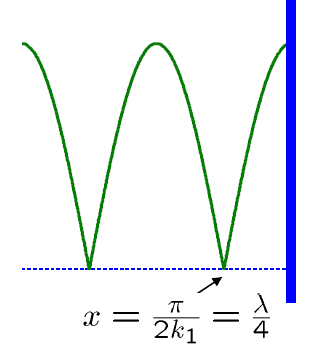
\includegraphics[scale=0.32]{acoustics/ch4/5}
	\captionof{figure}{}
	\label{fig:4.5}
	\end{minipage}		
	\begin{minipage}{0.25\textwidth}
	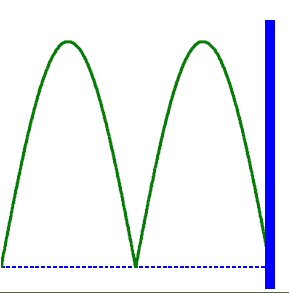
\includegraphics[scale=0.4]{acoustics/ch4/6}
	\captionof{figure}{}
	\label{fig:4.6}
	\end{minipage}		
	\end{center}
	
	\begin{wrapfigure}[10]{l}{5cm}
	\vspace{-5mm}
	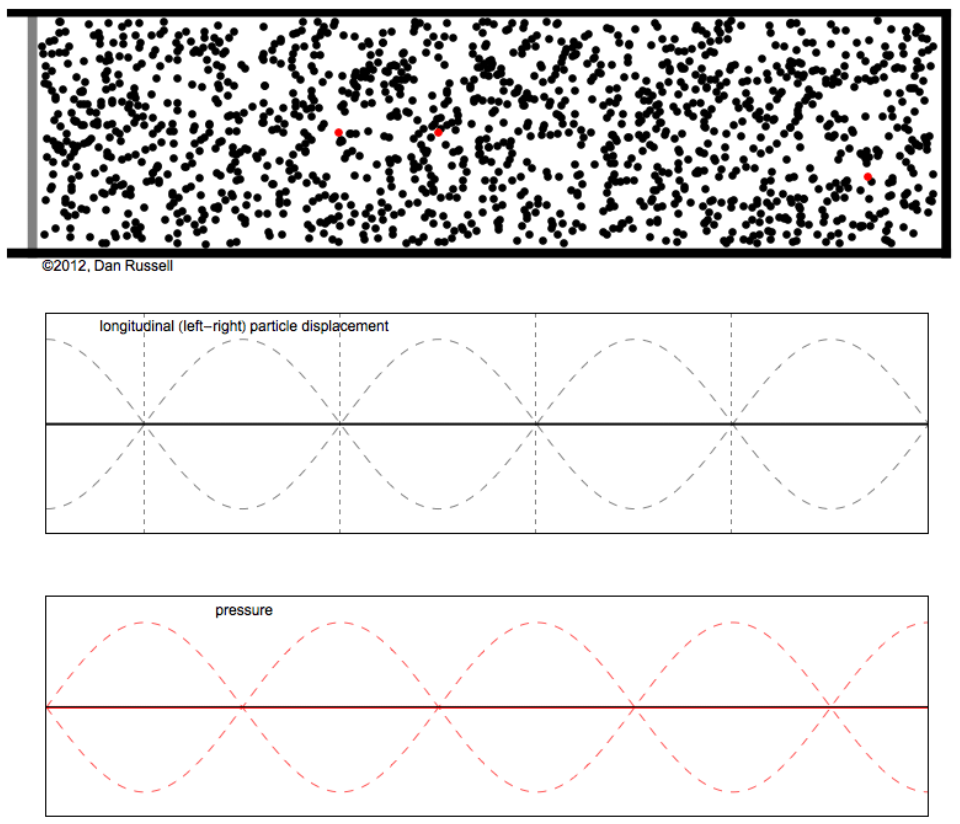
\includegraphics[scale=0.2]{acoustics/ch4/7}
	\captionof{figure}{}
	\label{fig:4.7}
	\end{wrapfigure}
	In practice, the amplitude of the pressure is maximum at the very right. The red particle has a maximum velocity, but the pressure is 0. In order to generate an acoustic mode, we need a source to generate a first signal. So at the very left we have a maximum velocity and 0 pressure. What I could have done instead of using a vibrating plate I could generate a sound in the cavity. The velocity would be 0 at both the wall, every $lambda/4$ I have the velocity 0 and pressure max. If I have the $L= \lambda n / 4$ n not even number, I will end up with the same scenario of this slide.
	
\section{Sound field in an enclosure}
	We assumed a wave propagating in 1D, but we can do the same in 3D: 
	
	\begin{equation}
	f_n = \frac{c}{2} \sqrt{\left(\frac{n_x}{l_x}\right)^2+ \left(\frac{n_y}{l_y}\right)^2 + \left(\frac{n_z}{l_z}\right)^2}.
	\end{equation}		
	
	 \begin{wrapfigure}[9]{r}{2cm}
	\vspace{-5mm}
	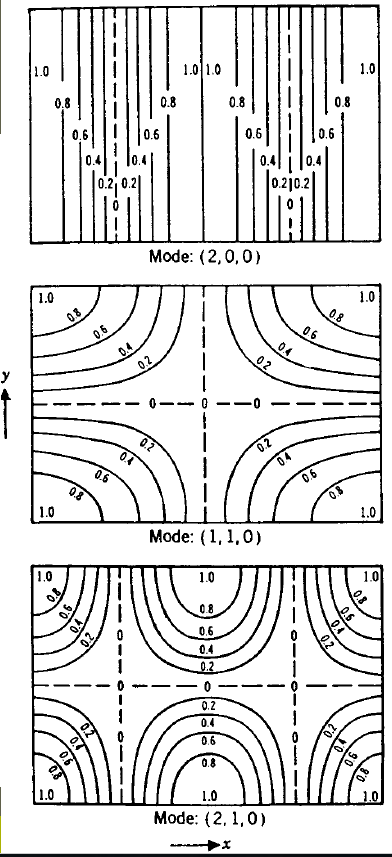
\includegraphics[scale=0.2]{acoustics/ch4/8}
	\captionof{figure}{}
	\label{fig:4.8}
	\end{wrapfigure}
	This equation is nothing else but $l = \lambda /2$. Indeed, if we consider only one direction, end up with $f = c/2l$. The $n_x$ .. are the mode numbers. The figure represents what happens in the different mode representations. On the first figure e represent a mode only in $n_x$, the second is a combination of 2 modes, we have 0 pressure at the center and max on the corners. The pressure field is:
	
	\begin{equation}
	p = \cos \frac{\pi n_x x}{l_x}\cos \frac{\pi n_y y}{l_y}\cos \frac{\pi n_z z}{l_z} e^{j\omega _n t}
	\end{equation}
	\ \\\\\\
	
	\begin{wrapfigure}[7]{l}{6cm}
	\vspace{-5mm}
	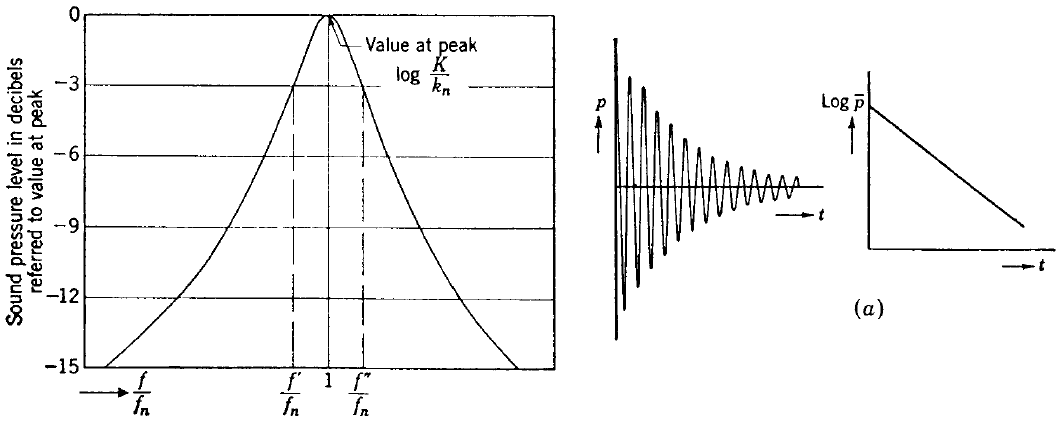
\includegraphics[scale=0.2]{acoustics/ch4/9}
	\captionof{figure}{}
	\label{fig:4.9}
	\end{wrapfigure}
	One thing that we change is the damping value when absorption. We have a maximum sound pressure amplitude in the resonance frequency and if it differs we have an amplitude smaller. This value can be related to geometric parameters of the room, S, V and the absorption coefficient of the material attached to the wall. In the time domain it looks like a sinus but decreasing, this decrease is characterized by: 
	
	\begin{equation}
	k_n = \frac{cSa}{8V} \qquad p_n = \frac{K}{k_n} e^{-k_n t} \cos (\omega _n t).
	\end{equation}
	
	Let's look to the frequencies where the resonance will happen. If the reflection is complete, the wavelength where this resonance happens is 2l. At which frequency? If I have a box of 1m 1m 1m so I have a $\lambda = 2$ so $f\lambda = c$ gives 170 Hz. 10m gives 17Hz and 10cm gives 1700Hz. That means that in large rooms, this acoustic resonance is not a problem, because the frequency is very low, we are talking about reflection in the wall so the sound loose its energy till reaching the wall. In the 1m the resonance is very hearable (0.1 not) that's exactly in the sensitive hearing range. \\
	
	How does a sound field look like in the neighbourhood of walls, standing waves. If I have a source in the middle of the room, I have spherical waves, and we given a certain sound power we can calculate the $L_p = L_w - 10\log S$. What will happen is that we don't have only the direct sound (from the source to the receiver) we have also the sound propagating indirectly, the one reflected on the wall, the sound pressure will be higher than the one I predicted with the formula. Outdoor (free field) this formula is valid but indoor not:
	
	\begin{equation}
	p_{eff}^2 = \frac{\rho c W}{4 \pi r^2}.
	\end{equation}	 
	
\subsubsection{Reverberating field}
	The additional sound power can be noted as the sum of the power absorbed by the walls. This intensity is moreover equal in the entire room:
	
	\begin{equation}
	W = \sum _i I_i a_i S_i = \bar{I} \sum _i a_i S_i = \bar{I} A = \frac{p_{eff}^2}{4\rho c} A \qquad \Rightarrow p_{eff}^2 = \frac{4\rho c W}{A}
	\end{equation}	 
	
	We have the surface of a certain wall and the absorption coefficient, I can write this as being A, the total absorption, unit of this is $m^2$. We call this, absorption in $m^2$ of open window. The best absorption is obtained when the window is open. We don't have any more the $\rho c$, but $4 \rho c$, because now I spread in the all direction and not in one direction, we will not show its math. In dB this gives:
	
	\begin{equation}
	L_p = 10 \log \left( \frac{p^2_{eff}}{p^2_0} \right) = 10 \log \left( \frac{\rho c W_0W4}{p_0^2W_0A} \right) \approx L_W - 10 \log A +6dB.
	\end{equation}

	Difuus sound because the intensity is supposed equal on the directions and the propagation is random. Which is the most important? The one direct or difuus? It depends, for small radius the direct term is high but for big radius the other term is bigger. Low absorbtion => low A => big term. In the case of A too small we will have standing wave in the room so I hear but 1m next not, we have to find the perfect A.